
\paragraph{About map} In book \cite{book}, a map is defined as a
continuous function (page 32), which is confusing. In this note, I
will not use this convention and will always states continuity
clearly.

\paragraph{Basic facts about maps}
Assuming domain $f=X$, codomain $f=Y$.
\begin{align}
    f(U\cup V) &= f(U)\cup f(V) \\
    f(U\cap V) &\subseteq f(U)\cap f(V) \\
    f(U^c) &\supseteq f(U)^c,\,\text{i.e. } f(U)^c \subseteq f(U^c) \\
    f^{-1}(U\cup V) &= f^{-1}(U)\cup f^{-1}(V) \\
    f^{-1}(U\cap V) &= f^{-1}(U)\cap f^{-1}(V) \\
    f^{-1}(U^c) &= [f^{-1}(U)]^c
\end{align}
\paragraph{Smallest the Largest Topolgy}
The set of all possible topolgies on $X$ is partially ordered by
inclusion. For a certain characteristics $\mathcal{C}$, it is possible
to have the smallest or the largest one. 

The \nomen{smallest topolgy} $\mathcal{T}_\text{min}$ is the one such
that, for any $\mathcal{T}'$ satisfying $\mathcal{C}$,
$\mathcal{T}_\text{min}\subseteq \mathcal{T}'$. The \nomen{largest
topolgy} $\mathcal{T}_\text{max}$ is the one such that, for any
$\mathcal{T}'$ satisfying $\mathcal{C}$, $\mathcal{T}'\subseteq
\mathcal{T}_\text{max}$.
Synonyms of these two words are:
\begin{itemize}
    \item Larger: stronger, finer.
    \item Smaller: weaker, coarser.
\end{itemize}
\begin{figure}[H]
    \centering
    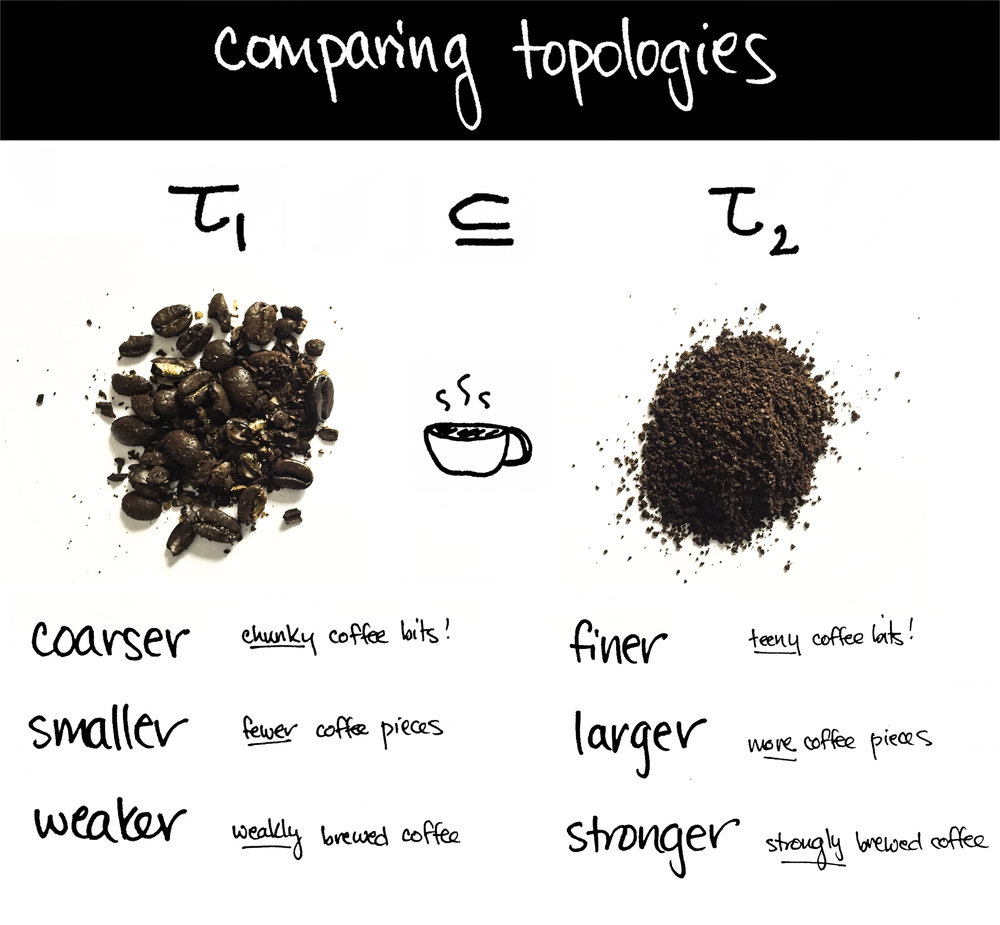
\includegraphics[width=0.65\linewidth]{pics/comparing-topologies-and-coffee.jpg}
    \caption{Comparing topologies and coffee (Credit:
    \href{http://www.math3ma.com/the-back-pocket/2016/8/26/comparing-topologies}{math3ma})}
\end{figure}
For example, assuming we have
\begin{equation}
    f: X\to Y
\end{equation}
where $f$ is any function.

If $X$ has topolgy $\mathcal{T}_X$, we ask then what kind of topolgy on
$Y$ will make $f$ a continuous function. First, all $f^{-1}(V)$, with
$V\in \mathcal{T}_Y$ should be open in $X$. So, the easiest choice is to
make $\mathcal{T}_{Y,\text{min}}=\{\varnothing,Y\}$, this is the
smallest topolgy.  Also, any set $V\in Y$ such that $f^{-1}(V)\notin
\mathcal{T}_X$ should not be in $\mathcal{T}_Y$. Then the largest
topolgy is $\mathcal{T}_{Y,\text{max}}=\{ V\subset Y| f^{-1}(V)\in
\mathcal{T}_X\}$.

If $Y$ has topolgy $\mathcal{T}_Y$, we also ask what kind of topolgy
on $X$ will make $f$ a continuous function. First, all $V\in
\mathcal{T}_Y$, their preimage $f^{-1}(V)$ must be in $\mathcal{T}_X$.
So the smallest topolgy is
$\mathcal{T}_{X,\text{min}}=\{f^{-1}(V)|V\in\mathcal{T}_Y\}$. Than
what about the largest topolgy? We consider, what kind of sets cannot
be inside $\mathcal{T}_X$. First, can $(f^{-1}(V))^c=f^{-1}(V^c)$ be
in $\mathcal{T}_X$? Yes. Since unless the space is connected, there
can be sets being both open and closed (other than $X$ and
$\varnothing$). Any other restrictions? No that I can think of. So,
the largest topolgy $\mathcal{T}_{X,\text{max}}=2^X$, the set of all
subsets of $X$. (The notation \nomen{$2^X$} is taken from the page 4
of book \cite{Singer.Thorpe}.

A summary:
\begin{table}[H]
    \centering
    \caption{Largest and Smallest Topolgies}
    \begin{tabular}{c l l}
        $X\overset{f}{\to}Y$ & Smallest  &Largest \\
        \hline
        Given $\mathcal{T}_X$ & $\mathcal{T}_{Y,\text{min}}=\{\varnothing,Y\}$        & $\mathcal{T}_{Y,\text{max}}=\{ V\subset Y| f^{-1}(V)\in \mathcal{T}_X\}$\\
        Given $\mathcal{T}_Y$ & $\mathcal{T}_{X,\text{min}}=\{f^{-1}(V)|V\in\mathcal{T}_Y\}$ & $\mathcal{T}_{X,\text{max}}=2^X$ \\
        No constraint & $\{\varnothing,X\}$ & $2^X$ \\
        \hline
    \end{tabular}
\end{table}
\paragraph{Facts about subspace/induced topolgy}
Let $Y$ be a subspace of a topological space $X$ wit induced topolgy.
\begin{fact}
    A set $H\subseteq Y$ is open in $Y$ if and only if $H=F\cap Y$
    for some open set $F$ in $X$.
\end{fact}
\begin{fact}
    A set $H\subseteq Y$ is closed in $Y$ if and only if $H=F\cap Y$
    for some closed set $F$ in $X$.
\end{fact}
\begin{fact}
    A set $H$ is open/closed in $X$ $\Rightarrow$ $H$ is open/closed
    in $Y$. But the converse may not be true. The converse statement
    depends on whether $Y$ is open or closed in $X$.
\end{fact}

\subsection{Lebesgue lamme}
\label{sec:Lebesgue lamme}

This is a very important lemma, which is why I gave it a seperate
section. It is labeled (3.11) in book \cite{book}.
\begin{thm}[Lebesgue Lemma]
    \label{thm:lebesgue-lemma} 
    Let $X$ be a compact metric space and let $\mathscr{F}$ be an open
    cover of $X$. Then there exists a real number $\delta>0$ (called
    the \nomen{Lebesgue number} of $\mathscr{F}$) such that any subset
    of $X$ of diameter less than $\delta$ is contained in some member
    of $\mathscr{F}$.
\end{thm}
